\documentclass[aspectratio=169,13pt]{beamer}

\usetheme{Madrid}
\usecolortheme{default}
\setbeamertemplate{navigation symbols}{}

\usepackage[utf8]{inputenc}
\usepackage[T1]{fontenc}
\usepackage{graphicx}
\usepackage{booktabs}
\usepackage{amsmath}
\usepackage{amssymb}
\usepackage{xcolor}
\usepackage{tikz}
\usetikzlibrary{positioning,shapes,arrows,calc}

\definecolor{DarkBlue}{RGB}{30, 57, 110}
\definecolor{LightBlue}{RGB}{173, 216, 230}
\definecolor{AccentRed}{RGB}{220, 50, 50}
\definecolor{AccentGreen}{RGB}{76, 175, 80}

\setbeamercolor{structure}{fg=DarkBlue}
\setbeamercolor{title}{fg=white,bg=DarkBlue}
\setbeamercolor{frametitle}{fg=white,bg=DarkBlue}
\setbeamercolor{block title}{fg=white,bg=DarkBlue}
\setbeamercolor{block body}{bg=LightBlue!20}

\title{Automated Mitosis Detection in Histopathology}
\subtitle{A Two-Stage Deep Learning Pipeline}
\author{Nihar Sagar G}
\institute{6th Semester - NNDL Course Project}

\begin{document}

% SLIDE 1: Title Page
\begin{frame}[plain]
  \titlepage
  \vspace{-0.8cm}
  \textcolor{DarkBlue}{\textbf{\large Dataset: TUPAC16}} \\
  \textcolor{DarkBlue}{\small Tumor Proliferation Assessment Challenge}
\end{frame}

% SLIDE 2: Motivation
\begin{frame}
  \frametitle{Motivation}
  \begin{columns}[T]
    \column{0.5\textwidth}
      \begin{block}{Clinical Problem}
        \begin{itemize}
          \item Mitosis count is key prognostic indicator
          \item Manual annotation is time-consuming
          \item High inter-observer variability
          \item Need for automated assessment
        \end{itemize}
      \end{block}
    
    \column{0.5\textwidth}
      \begin{block}{Technical Challenge}
        \begin{itemize}
          \item Mitotic figures are small (8--128 pixels)
          \item Class imbalance: many non-mitotic regions
          \item Domain shift across staining protocols
          \item Requires precise localization
        \end{itemize}
      \end{block}
  \end{columns}
\end{frame}

% SLIDE 3: Dataset Overview
\begin{frame}
  \frametitle{Dataset: TUPAC16}
  \begin{columns}[T]
    \column{0.5\textwidth}
      \begin{block}{Data Characteristics}
        \begin{itemize}
          \item \textbf{Source:} TUPAC16 Challenge
          \item \textbf{Training:} 8 slides
          \item \textbf{Validation:} 6 held-out slides
          \item \textbf{Multiple Centers:} Different scanners
          \item \textbf{Resolution:} 40x magnification
        \end{itemize}
      \end{block}
    
    \column{0.5\textwidth}
      \begin{block}{Preprocessing}
        \begin{itemize}
          \item Macenko color normalization
          \item Stage 1: $64 \times 64$ patches
          \item Stage 2: $512 \times 512$ patches
          \item Total: 600 annotated mitoses
          \item 80\% background patches excluded
        \end{itemize}
      \end{block}
  \end{columns}
\end{frame}

% SLIDE 4: Architecture Overview
\begin{frame}
  \frametitle{Two-Stage Pipeline}
  \centering
  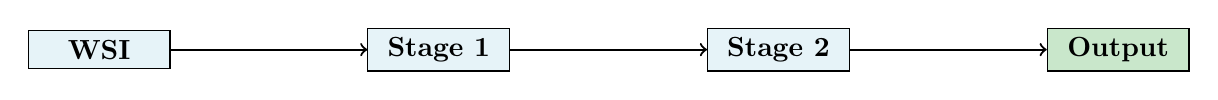
\begin{tikzpicture}[node distance=2.5cm]
    \node[draw, rectangle, fill=LightBlue!30, minimum width=1.8cm] (wsi) {\textbf{WSI}};
    \node[draw, rectangle, fill=LightBlue!30, minimum width=1.8cm, right=of wsi] (s1) {\textbf{Stage 1}};
    \node[draw, rectangle, fill=LightBlue!30, minimum width=1.8cm, right=of s1] (s2) {\textbf{Stage 2}};
    \node[draw, rectangle, fill=AccentGreen!30, minimum width=1.8cm, right=of s2] (out) {\textbf{Output}};
    
    \draw[->, thick] (wsi) -- (s1);
    \draw[->, thick] (s1) -- (s2);
    \draw[->, thick] (s2) -- (out);
  \end{tikzpicture}
  
  \vspace{1cm}
  \begin{columns}[T]
    \column{0.33\textwidth}
      \small \textbf{Input:} WSI tiles (40x)
    \column{0.33\textwidth}
      \small \textbf{Filter:} Binary classifier on $64 \times 64$
    \column{0.33\textwidth}
      \small \textbf{Detect:} R-CNN on $512 \times 512$
  \end{columns}
\end{frame}

% SLIDE 5: Stage 1 Classifier
\begin{frame}
  \frametitle{Stage 1: Binary Classifier}
  \begin{columns}[T]
    \column{0.5\textwidth}
      \begin{block}{Architecture}
        \begin{itemize}
          \item \textbf{Backbone:} EfficientNet-B3
          \item \textbf{Input:} $64 \times 64$ RGB patch
          \item \textbf{Output:} Binary probability
          \item \textbf{Loss:} Focal Loss
        \end{itemize}
      \end{block}
      \begin{block}{Loss Function}
        $$FL(p_t) = -\alpha(1-p_t)^{\gamma}\log(p_t)$$
        with $\gamma = 2$, $\alpha = 0.25$
      \end{block}
    
    \column{0.5\textwidth}
      \begin{block}{Performance}
        \begin{itemize}
          \item F1 Score: \textbf{0.8894}
          \item Precision: 0.92
          \item Recall: 0.87
          \item Epochs: 8
        \end{itemize}
      \end{block}
      \begin{block}{Threshold}
        $\tau = 0.5087$ (recall-optimized)
        \\ Flags $\sim$15\% of patches
      \end{block}
  \end{columns}
\end{frame}

% SLIDE 6: Stage 2 Detector
\begin{frame}
  \frametitle{Stage 2: Object Detector}
  \begin{columns}[T]
    \column{0.5\textwidth}
      \begin{block}{Architecture}
        \begin{itemize}
          \item \textbf{Model:} Faster R-CNN
          \item \textbf{Backbone:} ResNet50-FPN
          \item \textbf{Input:} $512 \times 512$ RGB
          \item \textbf{Output:} Bounding boxes
        \end{itemize}
      \end{block}
      \begin{block}{Custom Anchors}
        \begin{itemize}
          \item Sizes: 8, 16, 32, 64, 128 px
          \item For small objects
          \item Aspect ratios: 0.5, 1, 2
        \end{itemize}
      \end{block}
    
    \column{0.5\textwidth}
      \begin{block}{Performance}
        \begin{itemize}
          \item mAP@0.5: \textbf{0.7598}
          \item F1 Score: \textbf{0.7742}
          \item Precision: 0.714
          \item Recall: 0.789
          \item Epochs: 65
        \end{itemize}
      \end{block}
      \begin{block}{Inference}
        \begin{itemize}
          \item Confidence: 0.40
          \item NMS IoU: 0.3
        \end{itemize}
      \end{block}
  \end{columns}
\end{frame}

% SLIDE 7: Single-Center Results
\begin{frame}
  \frametitle{Results: Single-Center Performance}
  \centering
  \begin{tabular}{|c|c|c|c|}
    \hline
    \textbf{Config} & \textbf{F1} & \textbf{Prec} & \textbf{Status} \\
    \hline
    \rowcolor{}
    Stage 1 & 0.8894 & 0.92 & Screening \\
    \hline
    \rowcolor{}
    \textbf{Stage 2} & \textbf{0.7742} & \textbf{0.714} & \textbf{BEST} \\
    \hline
    Pipeline & 0.5806 & 0.68 & Not Rec. \\
    \hline
  \end{tabular}
  
  \vspace{0.8cm}
  \begin{alertblock}{Key Finding}
    Direct detection (F1=0.7742) outperforms cascade (F1=0.5806)!
    \\ Early filtering removes legitimate mitosis cases.
  \end{alertblock}
\end{frame}

% SLIDE 8: Cross-Center Generalization
\begin{frame}
  \frametitle{Cross-Center Evaluation: Domain Shift}
  \centering
  \begin{tabular}{|c|c|c|}
    \hline
    \textbf{Slide} & \textbf{Center} & \textbf{F1} \\
    \hline
    50 & A & 0.8571 \\
    67 & B & 0.8000 \\
    65 & C & 1.0000 \\
    66 & D & 1.0000 \\
    63 & E & 1.0000 \\
    \hline
    \rowcolor{AccentRed!30}
    34 & F & 0.2857 \\
    \hline
  \end{tabular}
  
  \vspace{0.8cm}
  \begin{alertblock}{\textbf{63\% F1 Degradation}}
    Different scanner/stain protocol on Slide 34 \\
    Critical for deployment: Multi-center validation essential
  \end{alertblock}
\end{frame}

% SLIDE 9: Error Analysis
\begin{frame}
  \frametitle{Error Analysis}
  \begin{columns}[T]
    \column{0.5\textwidth}
      \begin{block}{False Positives (3 total)}
        \begin{itemize}
          \item Overlapping nuclei
          \item Apoptotic bodies
          \item Stain artifacts
          \item Gallery: outputs/false\_positive\_gallery/
        \end{itemize}
      \end{block}
    
    \column{0.5\textwidth}
      \begin{block}{False Negatives (4 total)}
        \begin{itemize}
          \item Poorly stained figures
          \item Telophase mitosis
          \item Structure overlap
          \item Dataset disagreement
          \item Gallery: outputs/false\_negative\_gallery/
        \end{itemize}
      \end{block}
  \end{columns}
  
  \vspace{0.5cm}
\end{frame}

% SLIDE 10: Why Direct Detection Wins
\begin{frame}
  \frametitle{Why Direct Detection Beats Cascade}
  
  \begin{block}{Conventional Wisdom}
    Cascade reduces computation, Stage 1 filters easy negatives
  \end{block}
  
  \begin{alertblock}{Reality}
    Stage 1 threshold removes legitimate mitoses!
    \\ Some difficult but valid cases fall below $\tau = 0.5087$
  \end{alertblock}
  
  \begin{block}{Insight}
    For small object detection with class imbalance:
    \\ \textbf{End-to-end learning} $>$ Staged approaches
    \\ Deploy Stage 2 directly for best performance
  \end{block}
\end{frame}

% SLIDE 11: Pipeline Deployment
\begin{frame}
  \frametitle{End-to-End Pipeline}
  \begin{block}{Inference Workflow}
    \begin{enumerate}
      \item Load WSI at 40x magnification
      \item Sliding window: $512 \times 512$ patches
      \item Run Faster R-CNN (recommended)
      \item Slide-level NMS (IoU=0.3)
      \item Output: Bounding boxes + scores
      \item Nottingham score (clinical grading)
    \end{enumerate}
  \end{block}
  
  \vspace{0.3cm}
  \begin{block}{Nottingham Grading}
    \begin{itemize}
      \item Score 1: $\leq 7$ mitoses per 10 HPF
      \item Score 2: 8--14 mitoses per 10 HPF
      \item Score 3: $\geq 15$ mitoses per 10 HPF
    \end{itemize}
  \end{block}
\end{frame}

% SLIDE 12: Code Organization
\begin{frame}
  \frametitle{Code Organization}
  \small
  \begin{columns}[T]
    \column{0.5\textwidth}
      \begin{block}{Model Architecture}
        \texttt{models/}
        \begin{itemize}
          \small
          \item stage1\_classifier.py
          \item stage2\_detector.py
        \end{itemize}
      \end{block}
    
    \column{0.5\textwidth}
      \begin{block}{Training \& Inference}
        \texttt{src/}
        \begin{itemize}
          \small
          \item preprocess.py
          \item pipeline.py (run\_pipeline)
          \item evaluate.py
        \end{itemize}
      \end{block}
  \end{columns}
  
  \begin{block}{Entry Points}
    \begin{itemize}
      \small
      \item Train: \texttt{python src/stage2\_detector.py --mode train}
      \item Inference: \texttt{python src/pipeline.py --wsi\_path slide.tif}
      \item Interactive: \texttt{python gradio\_demo.py}
    \end{itemize}
  \end{block}
\end{frame}

% SLIDE 13: Interactive Demo - Gradio
\begin{frame}
  \frametitle{Try It Online: Gradio Demo}
  
  % \begin{block}{Interactive Web Interface}
  %   \begin{itemize}
  %     \item Upload histopathology images
  %     \item Real-time predictions
  %     \item Visual bounding box overlays
  %     \item Confidence scores per detection
  %   \end{itemize}
  % \end{block}
  \begin{columns}[T]
    \column{0.5\textwidth}
      \begin{block}{How to Run}
        \texttt{python gradio\_demo.py}
        
        \vspace{0.3cm}
        Opens web UI at:
        \\ \texttt{http://0.0.0.0:7861}
        
        \vspace{0.5cm}
        \textbf{Features}
        \begin{itemize}
          \small
          \item Upload WSI patches
          \item View annotated results
          \item Download predictions
          \item Mitosis counting
          \item Nottingham score
          \item Browser-based
          \item No terminal needed
        \end{itemize}
      \end{block}
    
    \column{0.5\textwidth}
      \begin{figure}
        \centering
        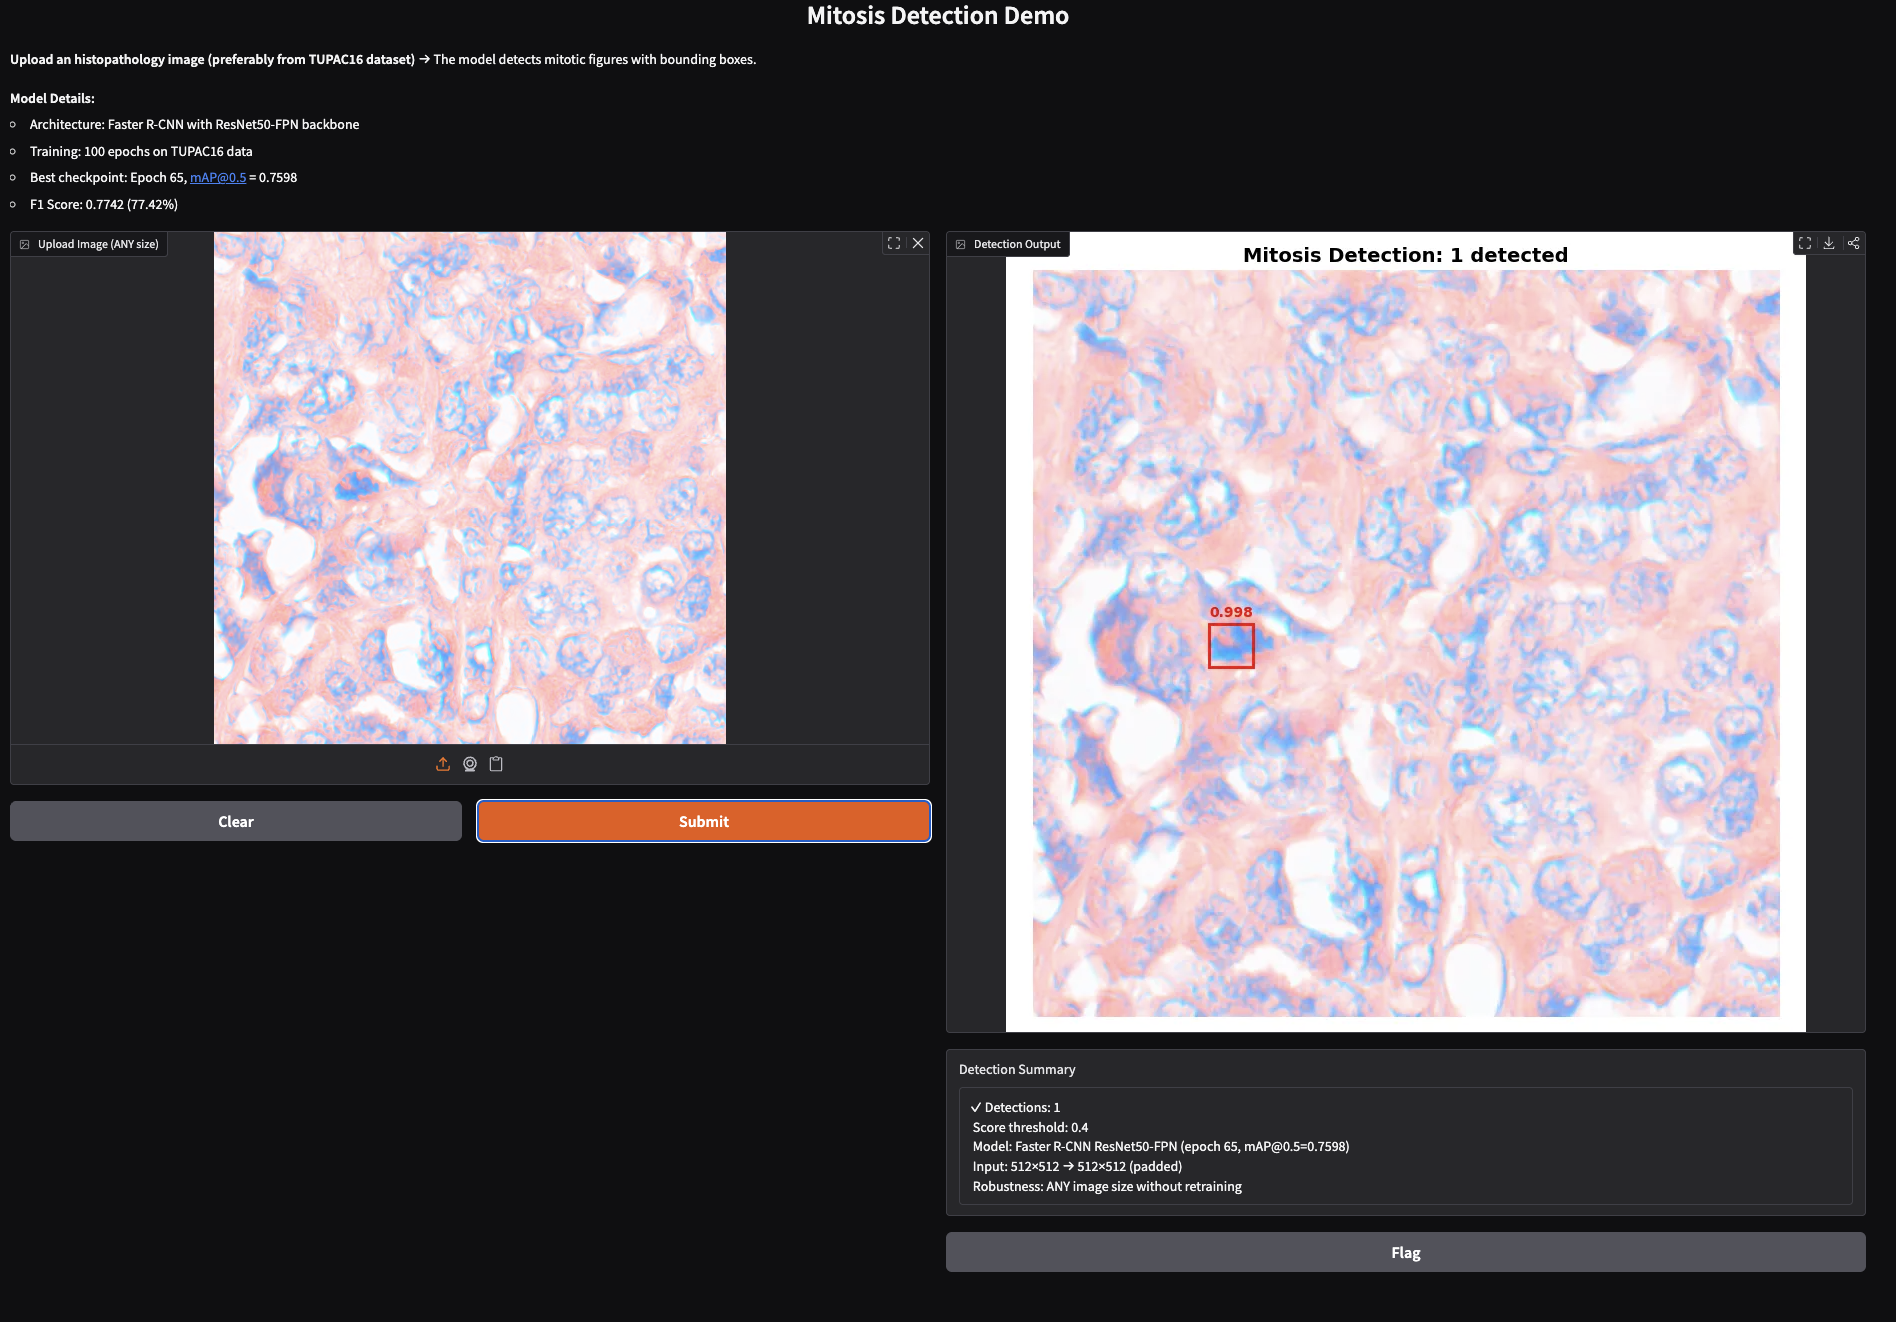
\includegraphics[width=0.9\linewidth]{image.png}
        \caption{\small Website Demo Interface}
      \end{figure}
  \end{columns}

\end{frame}

% SLIDE 14: Limitations and Future Work
\begin{frame}
  \frametitle{Limitations \& Future Work}
  \begin{columns}[T]
    \column{0.5\textwidth}
      \begin{block}{Current Limitations}
        \begin{itemize}
          \item Domain shift: 63\% F1 drop
          \item Single-center training
          \item Limited generalization
        \end{itemize}
      \end{block}
    
    \column{0.5\textwidth}
      \begin{block}{Future Directions}
        \begin{itemize}
          \item Domain adaptation
          \item Stain augmentation
          \item Ensemble methods
          \item Multi-center trial
          \item Explainability (Grad-CAM)
        \end{itemize}
      \end{block}
  \end{columns}
\end{frame}

% SLIDE 15: Key Takeaways
\begin{frame}
  \frametitle{Key Takeaways}
  
  \begin{block}{\large 1. Empirical Finding}
    Direct detection outperforms cascade \\
    F1: 0.7742 vs 0.5806
  \end{block}
  
  \begin{block}{\large 2. Domain Generalization}
    63\% F1 degradation on unseen stain \\
    Multi-center validation essential
  \end{block}
  
  \begin{block}{\large 3. Best Practices}
    \begin{itemize}
      \item Use Stage 2 only (F1=0.7742)
      \item Validate on your staining protocol
      \item Error analysis guides improvements
      \item Focal Loss + custom anchors matter
    \end{itemize}
  \end{block}
\end{frame}

% SLIDE 16: Conclusion
\begin{frame}
  \frametitle{Conclusion}
  
  \vspace{1cm}
  \centering
  \textcolor{DarkBlue}{\textbf{\Large Thank You!}}
  
  \vspace{0.5cm}
  \small
  GitHub: Mitosis-Detection-TUPAC16 \\
  Demo: Gradio (http://0.0.0.0:7861)
\end{frame}

% SLIDE 17: Appendix - Metrics
\begin{frame}
  \frametitle{Appendix: Evaluation Metrics}
  
  \begin{block}{Precision, Recall, F1}
    $$\text{Precision} = \frac{TP}{TP + FP}$$
    $$\text{Recall} = \frac{TP}{TP + FN}$$
    $$\text{F1} = 2 \cdot \frac{\text{Prec} \cdot \text{Recall}}{\text{Prec} + \text{Recall}}$$
  \end{block}
  
  \begin{block}{mAP and IoU}
    Mean Average Precision at IoU=0.5 \\
    IoU = $\frac{\text{Overlap}}{\text{Union}}$ threshold
  \end{block}
\end{frame}

% SLIDE 18: Appendix - Focal Loss
\begin{frame}
  \frametitle{Appendix: Focal Loss}
  
  \begin{block}{Standard Cross-Entropy}
    $$CE(p_t) = -\log(p_t)$$
  \end{block}
  
  \begin{block}{Focal Loss}
    $$FL(p_t) = -\alpha(1 - p_t)^{\gamma}\log(p_t)$$
  \end{block}
  
  \begin{block}{Key Properties}
    \begin{itemize}
      \item Down-weights easy negatives (high $p_t$)
      \item Focuses training on hard cases
      \item Addresses class imbalance
    \end{itemize}
  \end{block}
\end{frame}

\end{document}
